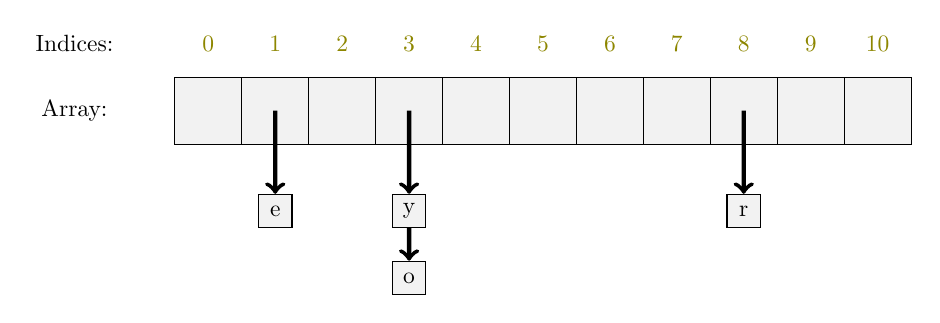
\begin{tikzpicture}[scale=0.85, transform shape]
	\foreach \x/\val in {0/,1/,2/,3/,4/,5/,6/,7/,8/,9/,10/}{
	\node[olive] (index) at (\x,1) {\x};
	\node[draw,rectangle, fill=gray!10, minimum size =1cm] (\x) at (\x,0) {\val};
}
\node[] at (-2,1) {Indices:};
\node[] at (-2,0) {Array:};

\node[draw,rectangle, fill=gray!10, minimum size =0.5cm] at (1,-1.5) (e) {e};
\node[draw,rectangle, fill=gray!10, minimum size =0.5cm] at (3,-1.5) (A) {y};
\node[draw,rectangle, fill=gray!10, minimum size =0.5cm] at (3,-2.5) (B){o};
\node[draw,rectangle, fill=gray!10, minimum size =0.5cm] at (8,-1.5) (r) {r};
\draw[->, ultra thick] (A) -- (B);
\draw[->, ultra thick] (1.center) -- (e);
\draw[->, ultra thick] (3.center) -- (A);
\draw[->, ultra thick] (8.center) -- (r);
\end{tikzpicture}
